\chapter{Desarrollo de infraestructura y servicios web}
Author es la plataforma de Seddi que permite a dise\~nadores, patronistas y dem\'as agentes involucrados en el proceso
de dise\~no y prototipado de una prenda trabajar con r\'eplicas digitales de tejidos sobre un entorno colaborativo web.\\

Un API REST proveee la informaci\'on de los tejidos capturados por Seddi para su representaci\'on en el contexto de Author,
que permite al usuario crear y editar patrones, detalles constructivos u ornamentos de una prenda. Este flujo permite
el dise\~no de una prenda completamente sobre el cliente web, mientras que para las acciones m\'as costosas, como la simulaci\'on
o renderizado basado en trazado de rayos se utilizan los servicios en la nube de Seddi.\\


\begin{figure}[H]
  \vspace{0.5cm}
  \centering
    \frame{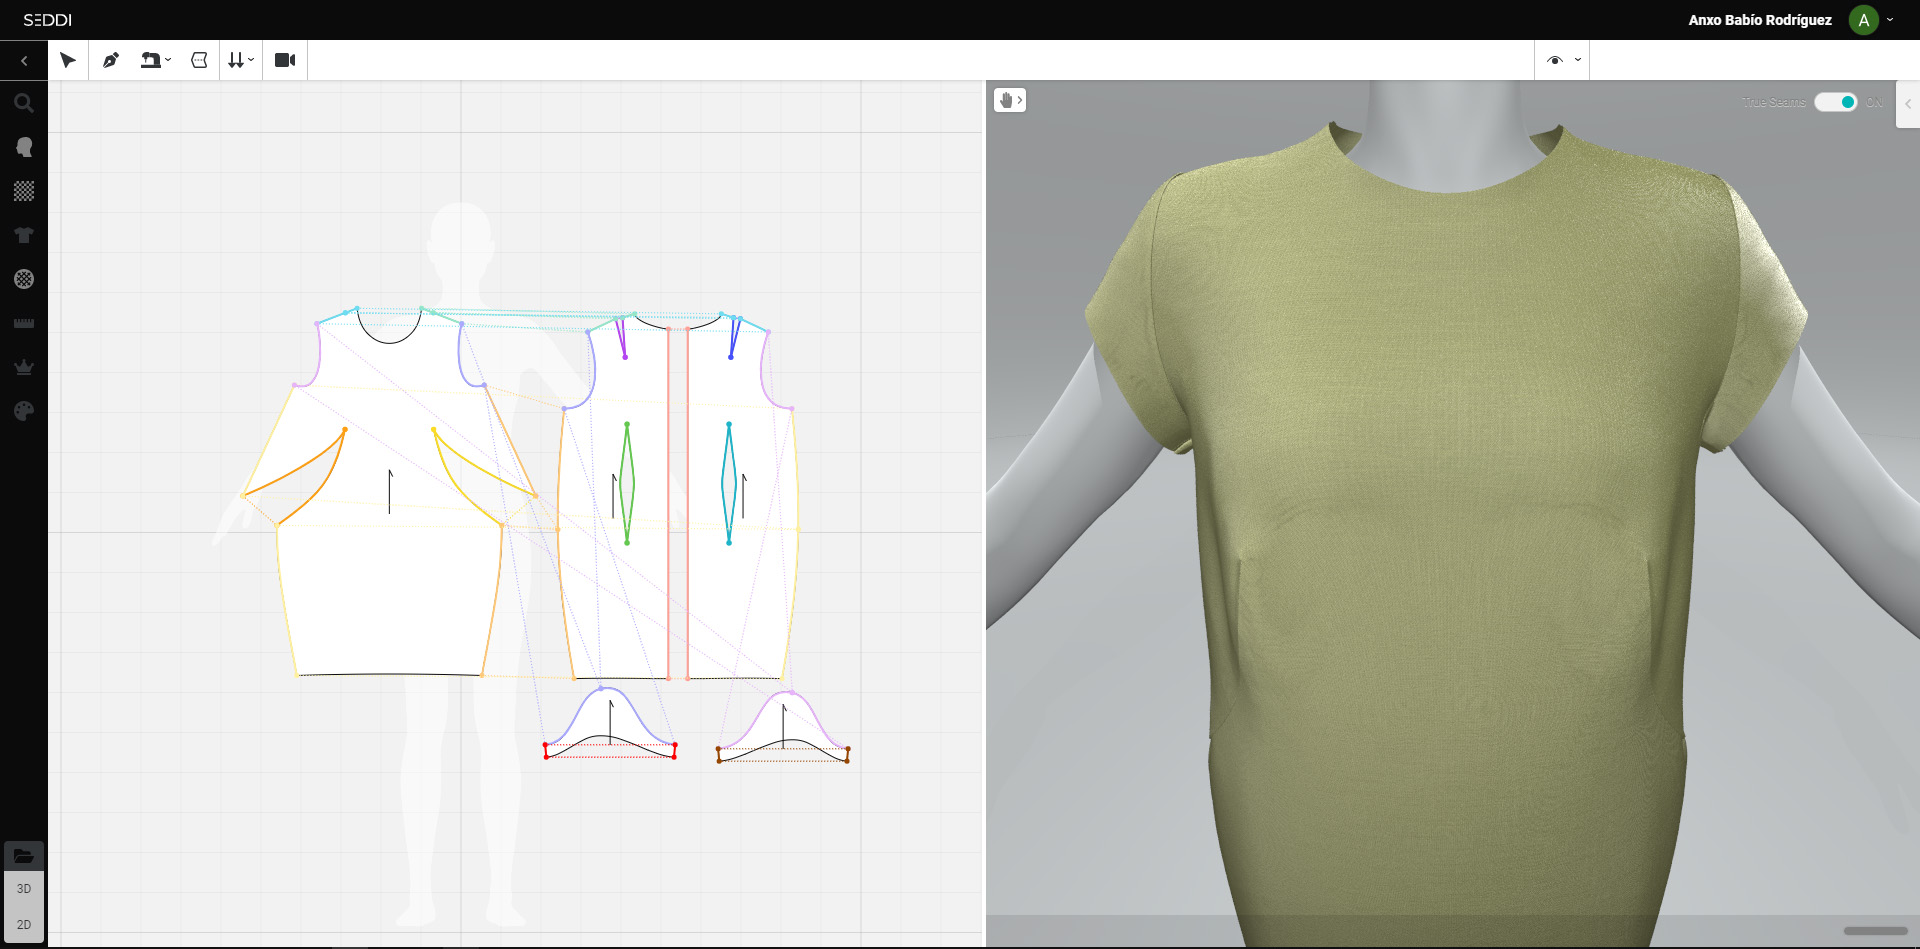
\includegraphics[scale=0.36]{viewports}}
  \caption{Editor de patrones 2D y editor 3D de Author}
\end{figure}

En la primera secci\'on de este cap\'itulo se detallan los cambios requeridos para dar soporte al nuevo modelo en la infraestructura
de Seddi. Por otra parte, la segunda secci\'on ofrece una visi\'on general del sistema de renderizado de ThreeJs, el motor de
renderizado que se utiliza en Author y sobre el que se integrar\'a el nuevo material.
% ofrece una visi\'on general sobre la arquitectura del sistema de renderizado de ThreeJs

% Para trabajar sobre estas r\'eplicas se proporcionan al usuario contextos 2D y 3D, as\'i como paneles de propiedades que
% permiten al usuario editar el patr\'on, detalles constructivos u ornamentos de una prenda. Este flujo permite el dise\~no
% y prototipado de la prenda completamente en el cliente web, mientras que para las acciones m\'as costosas, como la simulaci\'on
% o renderizado basado en trazado de rayos se utilizan los servicios en la nube de Seddi.\\

% Los servicios en la nube utilizan una arquitectura distribuida, diferentes servicios que se comunican entre s\'i para realizar
% una tarea en conjunto. Esta arquitectura implica una mayor complejidad, teniendo que comunicar los diferentes servicios,
% pero ofrece una mayor escalabilidad, tolerancia a fallos y la posibilidad de compartir recursos entre las partes del sistema.\\

% se computan en un servidor \textit{Hight Performance Computing} (HPC) que se reserva bajo demanda.\\

% y utiliza un sistema de cola
% de mensajes para recibir peticiones y enviar los resultados al cliente web

% El cliente web utiliza React para el desarrollo de UI, y ThreeJs y la API nativa de canvas para ofrecer un entorno interactivo.
% Author ofrece principalemente dos dos contextos, un entorno 2D que utiliza el API de canvas y en el que se pueden importar o
% editar patrones y un entorno 3D para previsualizar y editar detalles de disen\~no y constructivos de la prenda.

% Las interacciones de usuario actualizan el estado local del cliente que se comunica con el API REST para persistir los cambios
% sobre los recursos en base de datos. Este flujo permite el dise\~no y prototipado de la prenda completamente en el
% cliente web, mientras que para las acciones m\'as costosas, como la simulaci\'on o renderizado basado en trazado de rayos, se
% computan en un servidor \textit{Hight Performance Computing} (HPC) reservado bajo demanda.\\
% y utiliza un sistema de cola
% de mensajes para recibir peticiones y enviar los resultados al cliente web.

% Author es la plataforma web de Seddi que ofrece a los usuarios la posibilidad de trabajar con r\'eplicas digitales de los tejidos
% para dise\~nar prendas. Para ello se sirve de una infraestructura en la nube que proporciona acceso a los datos de tejidos
% capturados as\' y expone funcionalidades de las tecnolog\'ias de captura y simulaci\'on de Seddi.

% Al contrario que en una arquitectura centralizada, en la que la l\'ogica de negocio se controla en un sistema
% principal, los servicios en la nube utilizan una arquitectura distribuida, diferentes servicios que se comunican
% entre s\'i para realizar una tarea en conjunto. Esta arquitectura implica una mayor complejidad, teniendo que comunicar
% los diferentes servicios, pero ofrece una mayor escalabilidad, tolerancia a fallos y la posibilidad de compartir recursos
% entre las partes del sistema.\\

% Para trabajar con las r\'eplicas digitales de tejidos y tecnolog\'ias de simulaci\'on y renderizado desarrolladas por los
% departamentos de investigaci\'on de Seddi, la plataforma de Author se apoya en una infraestructura de servicios en la nube
% de Seddi.\\

% Los servicios gestionan una colecci\'on de recursos relacionados y exponen su funcionalidad a trav\'es de contratos a
% otros usuarios y servicios parte del sistema




% Las interacciones de usuario actualizan el estado local del cliente que se comunica con el API REST para persistir los cambios
% sobre los recursos en base de datos. Este flujo permite el dise\~no y prototipado de la prenda completamente en el
% cliente web, mientras que para las acciones m\'as costosas, como la simulaci\'on o renderizado basado en trazado de rayos, se
% computan en un servidor \textit{Hight Performance Computing} (HPC) que se reserva bajo demanda y utiliza un sistema de cola
% de mensajes para recibir peticiones y enviar los resultados al cliente web.




% Author es la plataforma web de Seddi que ofrece a los usuarios la posibilidad de trabajar con r\'eplicas digitales de los tejidos
% para dise\~nar prendas. Para ello se sirve de una infraestructura en la nube que proporciona acceso a los datos de tejidos
% capturados as\' y expone funcionalidades de las tecnolog\'ias de captura y simulaci\'on de Seddi.

% El cliente web utiliza React para el desarrollo de UI, y ThreeJs y la API nativa de canvas para ofrecer un entorno interactivo.
% Author ofrece principalemente dos dos contextos, un entorno 2D que utiliza el API de canvas y en el que se pueden importar o
% editar patrones y un entorno 3D para previsualizar y editar detalles de disen\~no y constructivos de la prenda.

% para
% permitir al usuario editar y consultar propiedades del tejido, detalles constructivos, ornamentos, etc. 


% Canvas de HTML para el editor 2D y Three.js como motor de renderizado para el editor de 3D. Las interacciones de
% usuario actualizan el estado local del cliente y se comunica con el API REST para persistir los cambios sobre
% los recursos en base de datos. Este flujo permite el dise\~no y prototipado de la prenda completamente en el
% cliente web, mientras que para las acciones m\'as costosas, como la simulaci\'on o renderizado offline de tejidos,
% se reserva al usuario un servidor que utiliza un servicio HPC de Seddi encarga de recibir, procesar y enviar la
% petici\'on a traves del sistema de cola de mensajes.

% \begin{figure}[H]
%   \vspace{1cm}
%   \centering
%     \frame{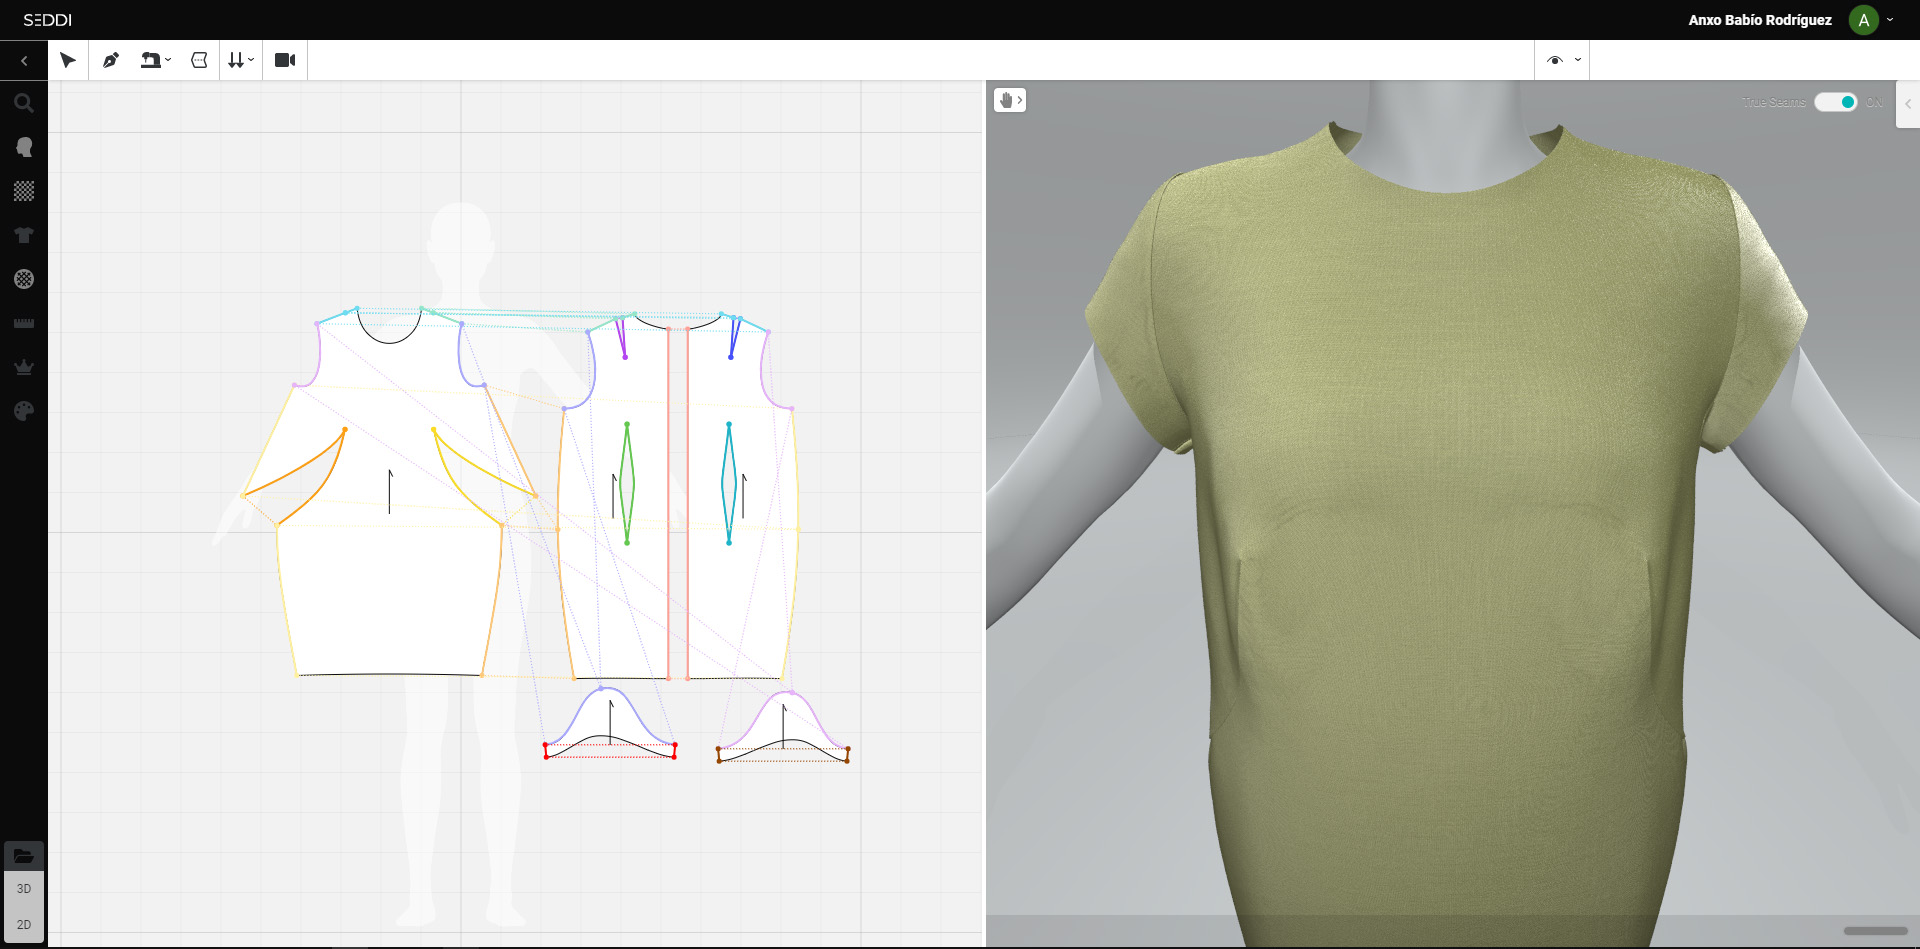
\includegraphics[scale=0.28]{viewports}}
%   \caption{Editor de patrones 2D y editor 3D de Author}
%   \vspace{0.5cm}
% \end{figure}

\section{Servicios en la nube de Seddi}

\bgroup

  Los servicios en la nube utilizan una arquitectura distribu\'ida, diferentes servicios que se comunican entre s\'i para realizar
  una tarea en conjunto. Esta arquitectura implica una mayor complejidad, teniendo que comunicar los diferentes servicios,
  pero ofrece una mayor escalabilidad, tolerancia a fallos y la posibilidad de compartir recursos entre las partes del sistema.

  \begin{figure}[H]
    \vspace{0.5cm}
    \centering
      \frame{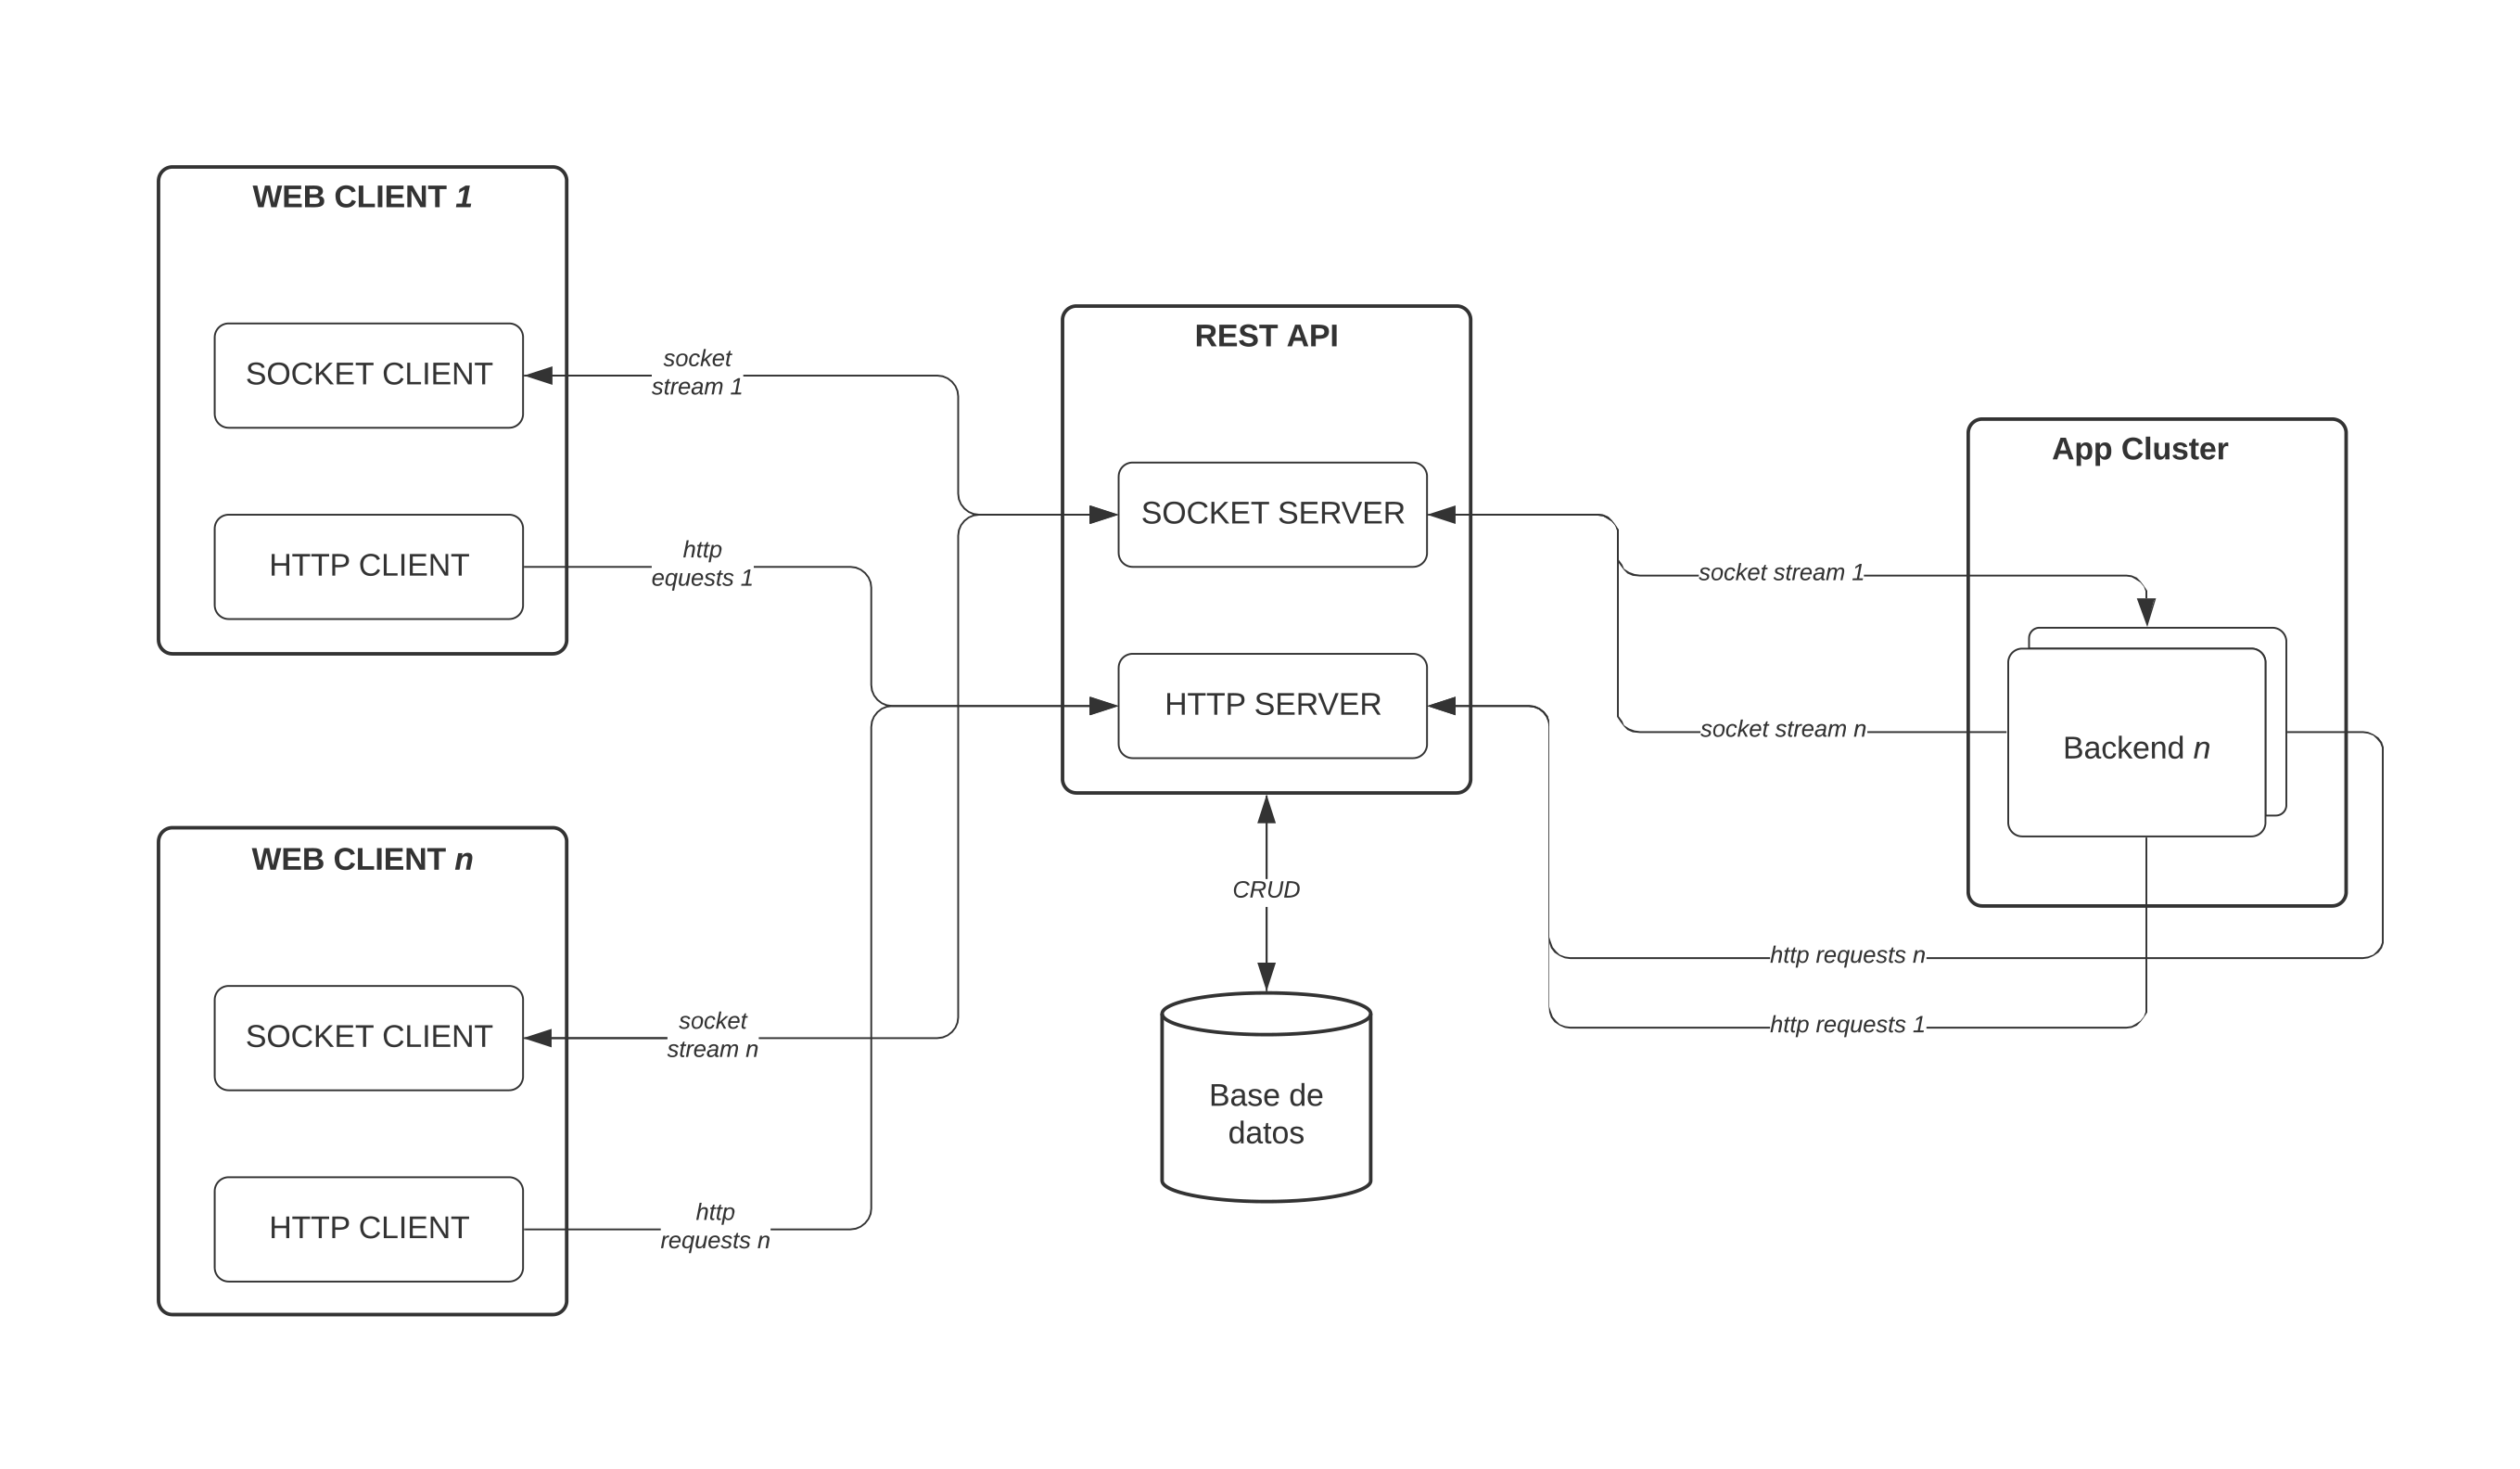
\includegraphics[scale=0.55]{seddi_diagram}}
    \caption{Esquema simplificado de comunicaciones y servicios en Seddi.}
    \vspace{0.5cm}
  \end{figure}

  Seddi ofrece sus servicios a trav\'es de clientes web que exponen la funcionalidad al usuario y se comunican con un API
  REST para gestionar el acceso a recursos compartidos en la plataforma. Para utilizar un nuevo material especializado en tejidos,
  adem\'as de actualizar el motor de renderizado, ha de actualizarse la infraestructura de servicios de Seddi para crear un modelo
  de datos que lo represente en el sistema de almacenamiento de Seddi, as\'i como proveer acceso a \'el a trav\'es del API
  REST. Por otra parte, las acciones m\'as costosas, como la simulaci\'on o el renderizado basado en trazado de rayos, se
  computan en servicios de \textit{Hight Performance Computing} (HPC) que se reservan bajo demanda.


  % la infraestructura ha de soportar su modelo de datos a dem\'as de proveer acceso a \'el a trav\'es del API REST.
  
  % Las operaciones m\'as costasas se ejecutan, bajo demandad,
  % en servicios de \textit{High Performance Computing} (HPC) utilizando un sistema de cola de mensajes.

  % y una conexion de sockets con un sistema de cola de
  % mensajes para pedir y recibir en tiempo real las operaciones graficas mas costosas que se realizan en los servidores en la nube.

\egroup

\subsection{Implementaci\'on del modelo de datos}
Como sistema de almacenamiento de datos Seddi utiliza MongoDB \autocite{mongodb}, un sistema NoSQL basado en documentos. Los sistemas no relacionales
nacieron a mediados de los 90 frente a los sistemas SQL y sus principales ventajas son sus bajos tiempos de respuesta, flexibilidad
en el modelo de datos y escalabilidad horizontal.\\

Para asegurar la consistencia entre los diferentes motores de la compa\~n\'ia, la representaci\'on de los materiales en base de
datos y las interfaces que proporcionan acceso a ellos son comunes. Adem\'as, los motores de renderizado utilizan un \textit{Entity Component System}
(ECS) \autocite{ecs}, las referencias a materiales se serializan como parte de un componente.\\

Los componentes que permiten renderizar elementos con materiales en la escena son \textit{GarmentPieceComponent} y \textit{MeshRenderableComponent}.
\textit{GarmentPieceComponent} se especializa en representar tejidos en la escena y \textit{MeshRenderableComponent}
se utiliza para definir el resto de elementos con materiales como escenarios, avatares, fornituras, etc.

\begin{figure}[H]
  \vspace{0.5cm}
  \centering
    \frame{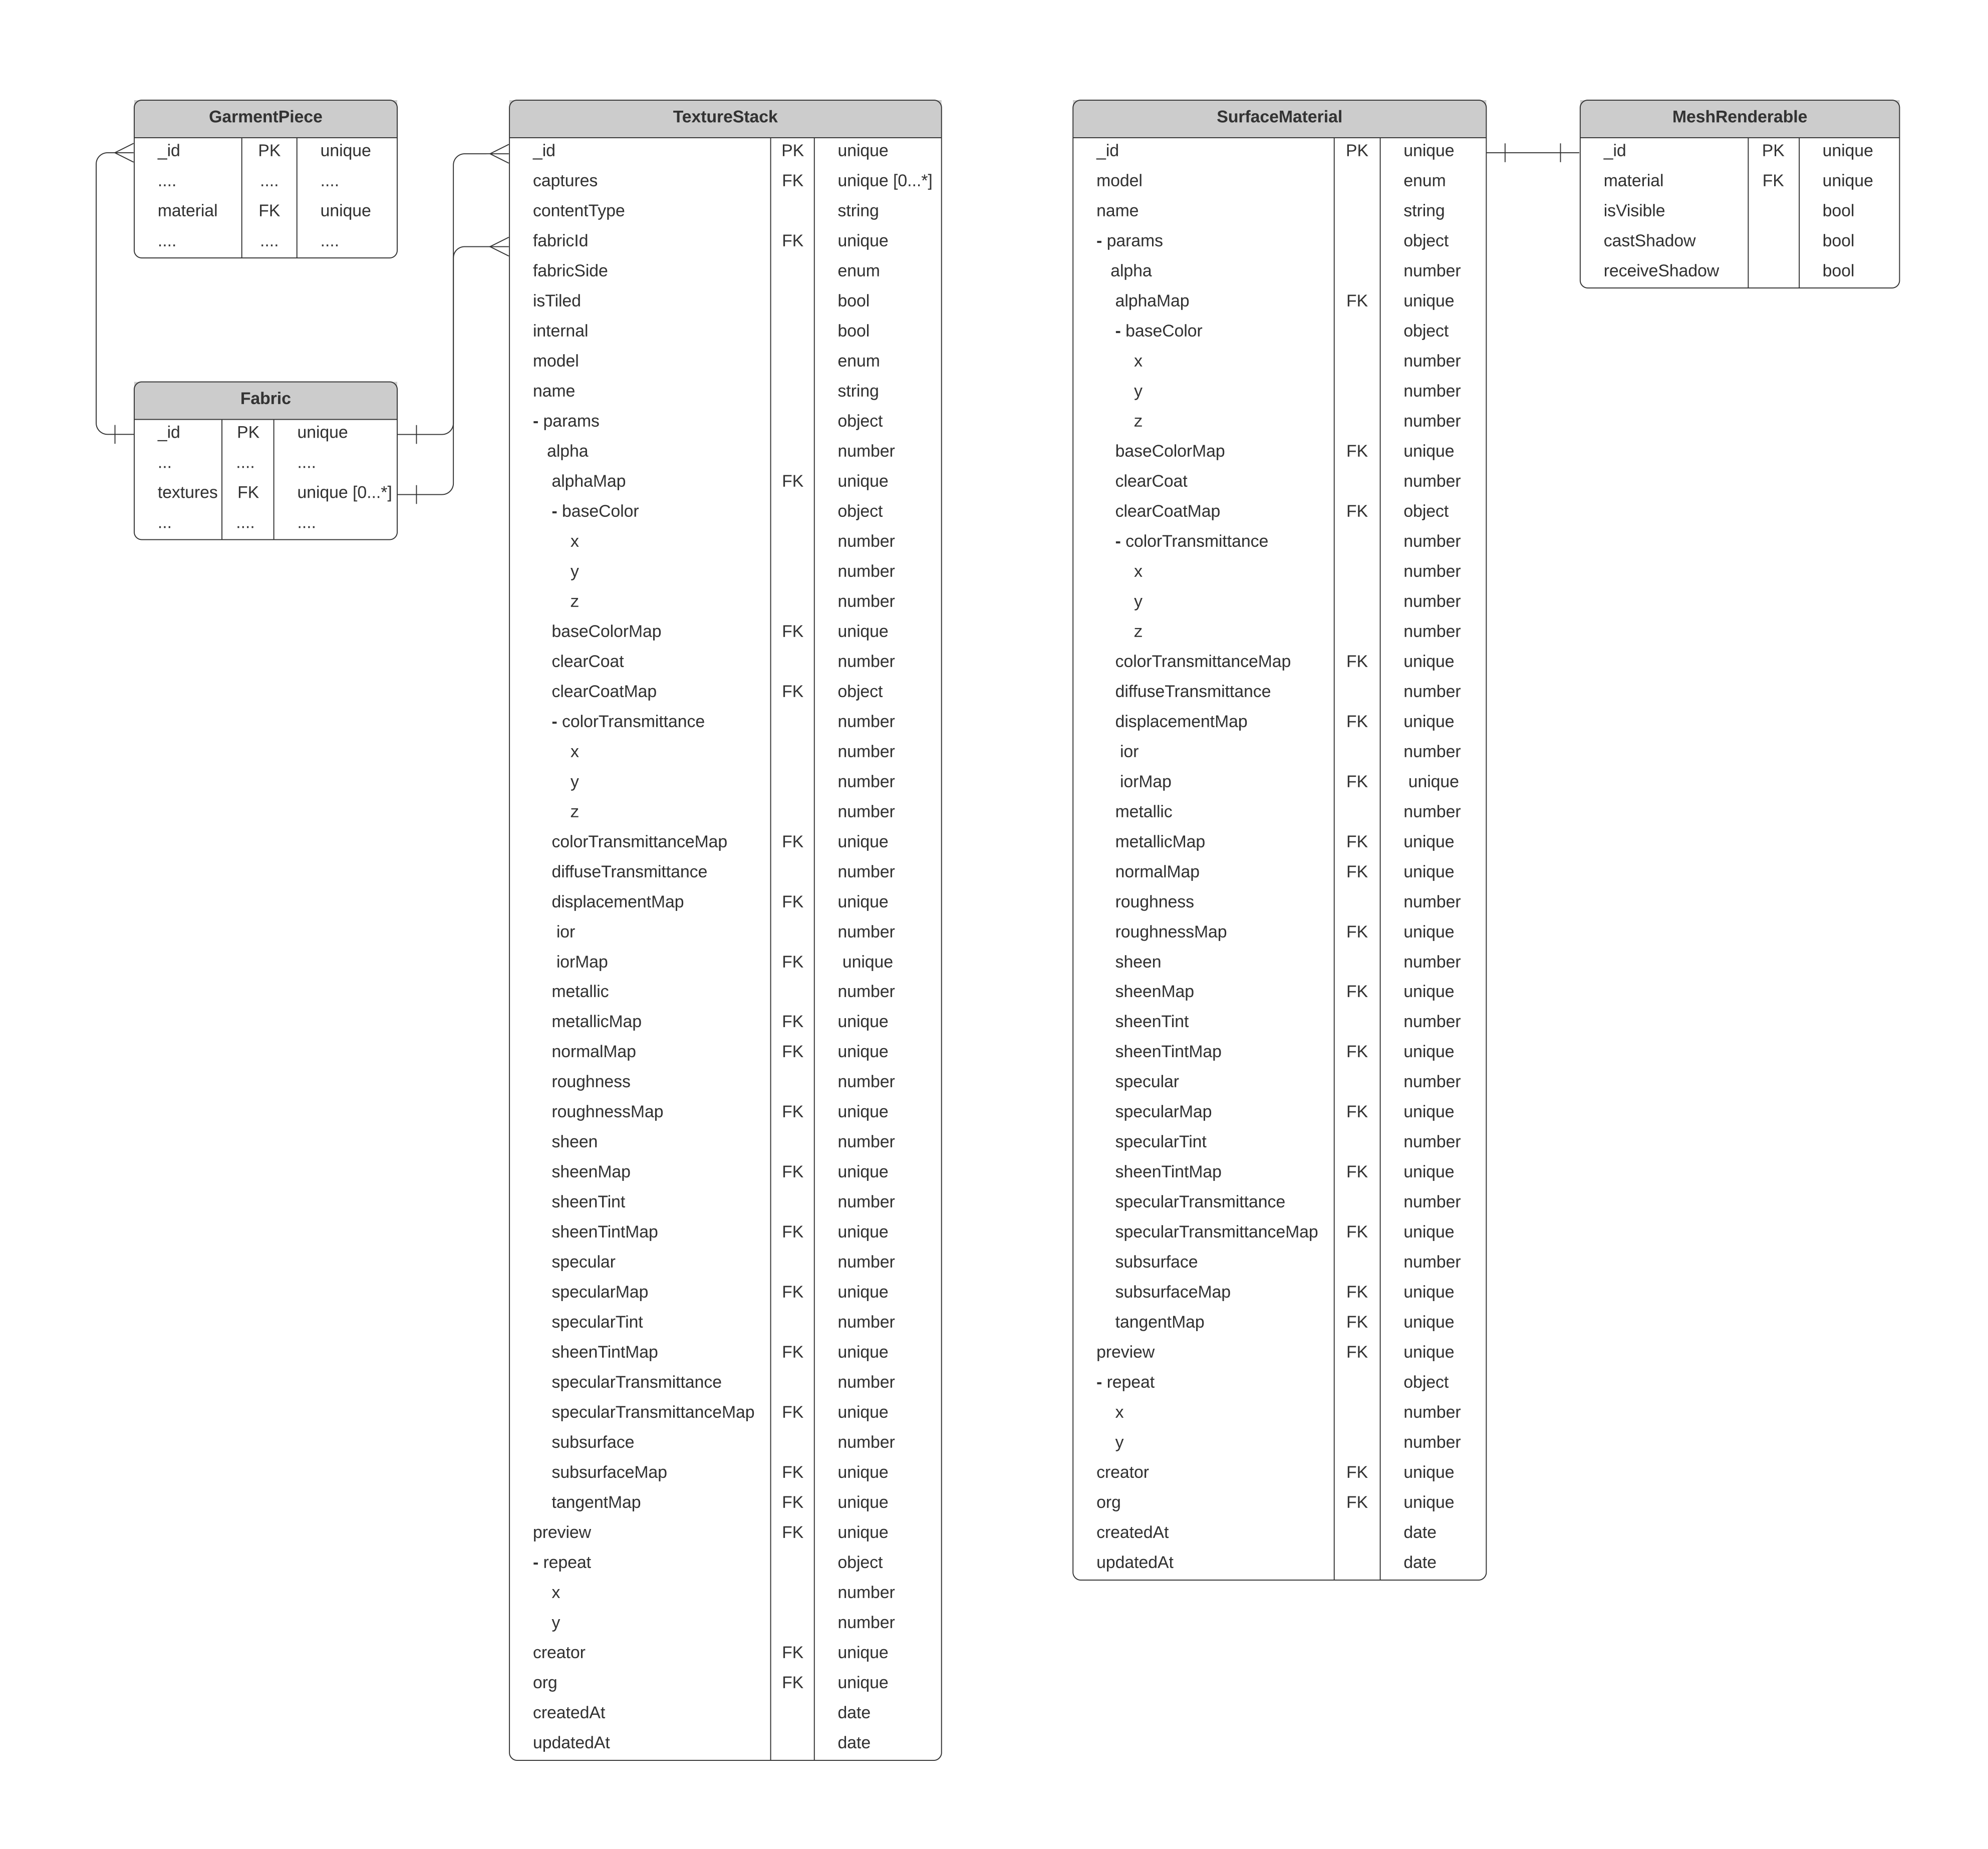
\includegraphics[scale=0.37]{materials_schema}}
  \caption{Modelo de datos de los recursos que soportan materiales.}
  \vspace{0.5cm}
\end{figure}

Los materiales de un \textit{GarmentPieceComponent} se almacenan en el campo \textit{textures} de un recurso \textit{Fabric}. El campo
\textit{textures} es un array que referencia recursos \textit{TextureStack} que contienen las definiciones de los materiales para
la parte frontal y trasera obtenidas durante el proceso de captura \'optica. Por otra parte, los materiales de un \textit{GarmentPieceComponent}
se almacenan en recursos \textit{SurfaceMaterial}. Estos recursos almacenan diferentes tipos de metadatos y pueden utilizar
diferentes modelos de BRDFs pero comparten la parametrizaci\'on de los materiales.

% Mientras que la
% representaci\'on de un material de \textit{GarmentPieceComponent} se almacena bajo el nombre de \textit{TextureStack} y es el
% resultada



% El modelo de datos que representa un material en la infraestructura de Seddi es com\'un a los diferentes motores de renderizado
% de la compa\~n\'ia, de esta forma los motores comparten parametrizaci\'on.

% La informaci\'on de un material para que los motores gr\'aficos del cliente web y los servicios de HPC
% se almacena en un \textit{TextureStack}, que son resultado de la captura \'optica de un tejido, o un \textit{SurfaceMaterial}, la definici\'on para
% cualquier otro elemento de la escena 3D. Ambos motores gr\'aficos utilizan un Entity Component System (ECS), por lo que
% la informacion sobre los materiales son una referencia un \textit{GarmentPieceComponent}, en el caso de un \textit{TextureStack},
% o un \textit{MeshRenderableComponent}, en el caso de un \textit{SurfaceMaterial}.\\



\subsection{Actualizaci\'on de las interfaces de servicios REST}
El API REST que proporciona acceso a los recursos est\'a montada sobre Node \autocite{node}, un entorno de ejecuci\'on de Javascript montado
sobre el motor V8 de Google que proporciona operaciones no bloqueantes de lectura y escritura (I/O) a disco o red.
De entre la variedad de \textit{frameworks} disponibles en el ecosistema de Node, el API REST de Seddi utiliza Express debido
a su amplia comunidad, rendimiento, facilidad y velocidad de desarrollo.\\

\begin{figure}[H]
  \vspace{0.5cm}
  \centering
    \frame{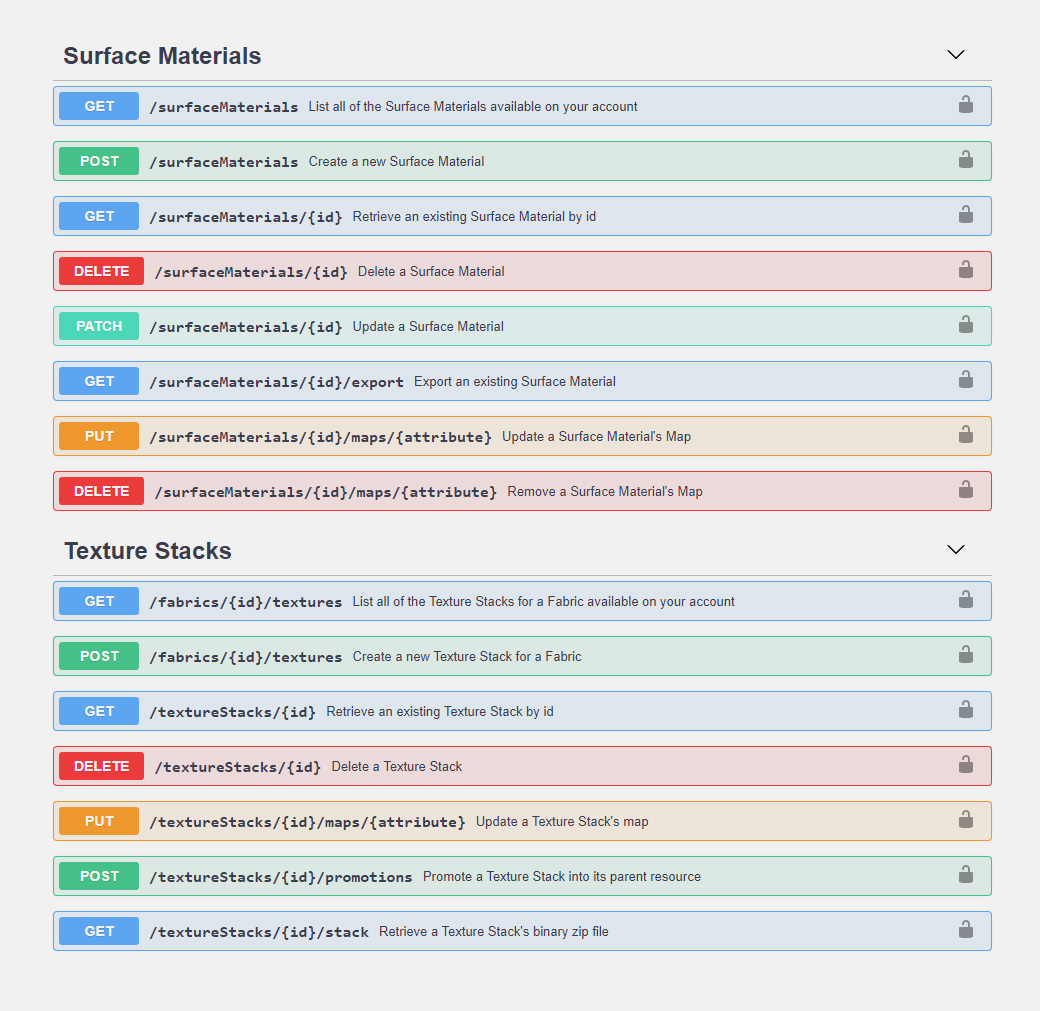
\includegraphics[scale=0.37]{swagger}}
  \caption{Documentaci\'on de los recursos SurafaceMaterial y TextureStack en Swagger.}
  \vspace{0.5cm}
\end{figure}

Las operaciones permitidas sobre los recursos \textit{SurfaceMaterial} y \textit{TextureStack} son: crear, obtener, actualizar y borrar
un recurso por \textit{id}, adem\'as de permitir actualizar la textura de un mapa y descargar la definici\'on del material
y sus texturas. Adicionalmente, un \textit{TextureStack} puede ser promocionado, lo que indica que el recurso indicado
es el que se utiliza dentro del campo \textit{textures} del \textit{Fabric} asociado, que se indica en el campo \textit{fabricId} del
\textit{TextureStack}.\\
\newpage
Las citadas funcionalidades se documentan en Swagger \autocite{swagger}, una herramienta de documentaci\'on automatizada que proporciona una gu\'ia a
a los consumidores del API.

% es la definici\'on
% de material que se utilizar\'a






\section{Motor de renderizado de Author}
% \todo[inline]{
%   % Para trabajar sobre estas r\'eplicas se proporcionan al usuario contextos 2D y 3D, as\'i como paneles de propiedades que
%   % permiten al usuario editar el patr\'on, detalles constructivos u ornamentos de una prenda.
%   Author ofrece un contexto interactivo de edici\'on que permite al usuario la edici\'on de y creaci\'on de patrones, detalles
%   constructivos u ornamentos de una prenda. La edici\'on se realiza a trav\'es de paneles de propiedades, y contextos de 2D
%   y 3D. Este trabajo se centra en el editor 3D para incrementar el realismo de los tejidos y su coherencia con las im\'agenes
%   generadas por el servicio de renderizado basado en trazado de rayos.\\

%   En esta secci\'on se ofrece una visi\'on general sobre la arquitectura de su sistema de renderizado,
%   su librer\'ia de materiales y los matem\'aticos e implementaciones utilizadas por sus materiales PBR.\\
% }
Adem\'as de actualizar el modelo de datos y las interfaces que ofrecen acceso a ellos, el nuevo material ha de ser integrado
dentro del contexto 3D basado en ThreeJs de Author. A continuaci\'on se analiza la arquitectura de su sistema de renderizado,
su librer\'ia de materiales y los modelos matem\'aticos e implementaciones utilizadas por sus materiales PBR.\\

% a\~nadiendo un nuevo material a su librer\'ia
% de materiales est\'andar. 
% Author ofrece dos entornos de edici\'on, un contexto 2D que utiliza el API de canvas y en el que se pueden importar o
% editar patrones y un contexto 3D para previsualizar y editar detalles
% de dise\~no y constructivos de la prenda.\\

% Este trabajo trata de incrementar el realismo del contexto 3D interactivo y mejorar la coherencia
% con el motor de renderizado bajo demanda basado en el trazado de rayos. Con intenci\'on de ofrecer una visi\'on amplia
% sobre ThreeJs, motor en el que se implementar\'a el nuevo modelo de material, 

% A continuaci\'on se explica la arquitectura y el sistema de materiales materiales de ThreeJs.


\subsection{Arquitectura del sistema de renderizado de ThreeJs}
El nuevo material extiende la librer\'ia de materiales para ofrecer una interfaz igual al resto de materiales nativos
de ThreeJs. Para ello, estudiaremos la arquitectura del motor de renderizado de ThreeJs tomando como referencia los dos
materiales disponibles en la librer\'ia, \textit{MeshStandardMaterial} y \textit{MeshPhysicalMaterial}.

\begin{figure}[H]
  \vspace{0.5cm}
  \centering
    \frame{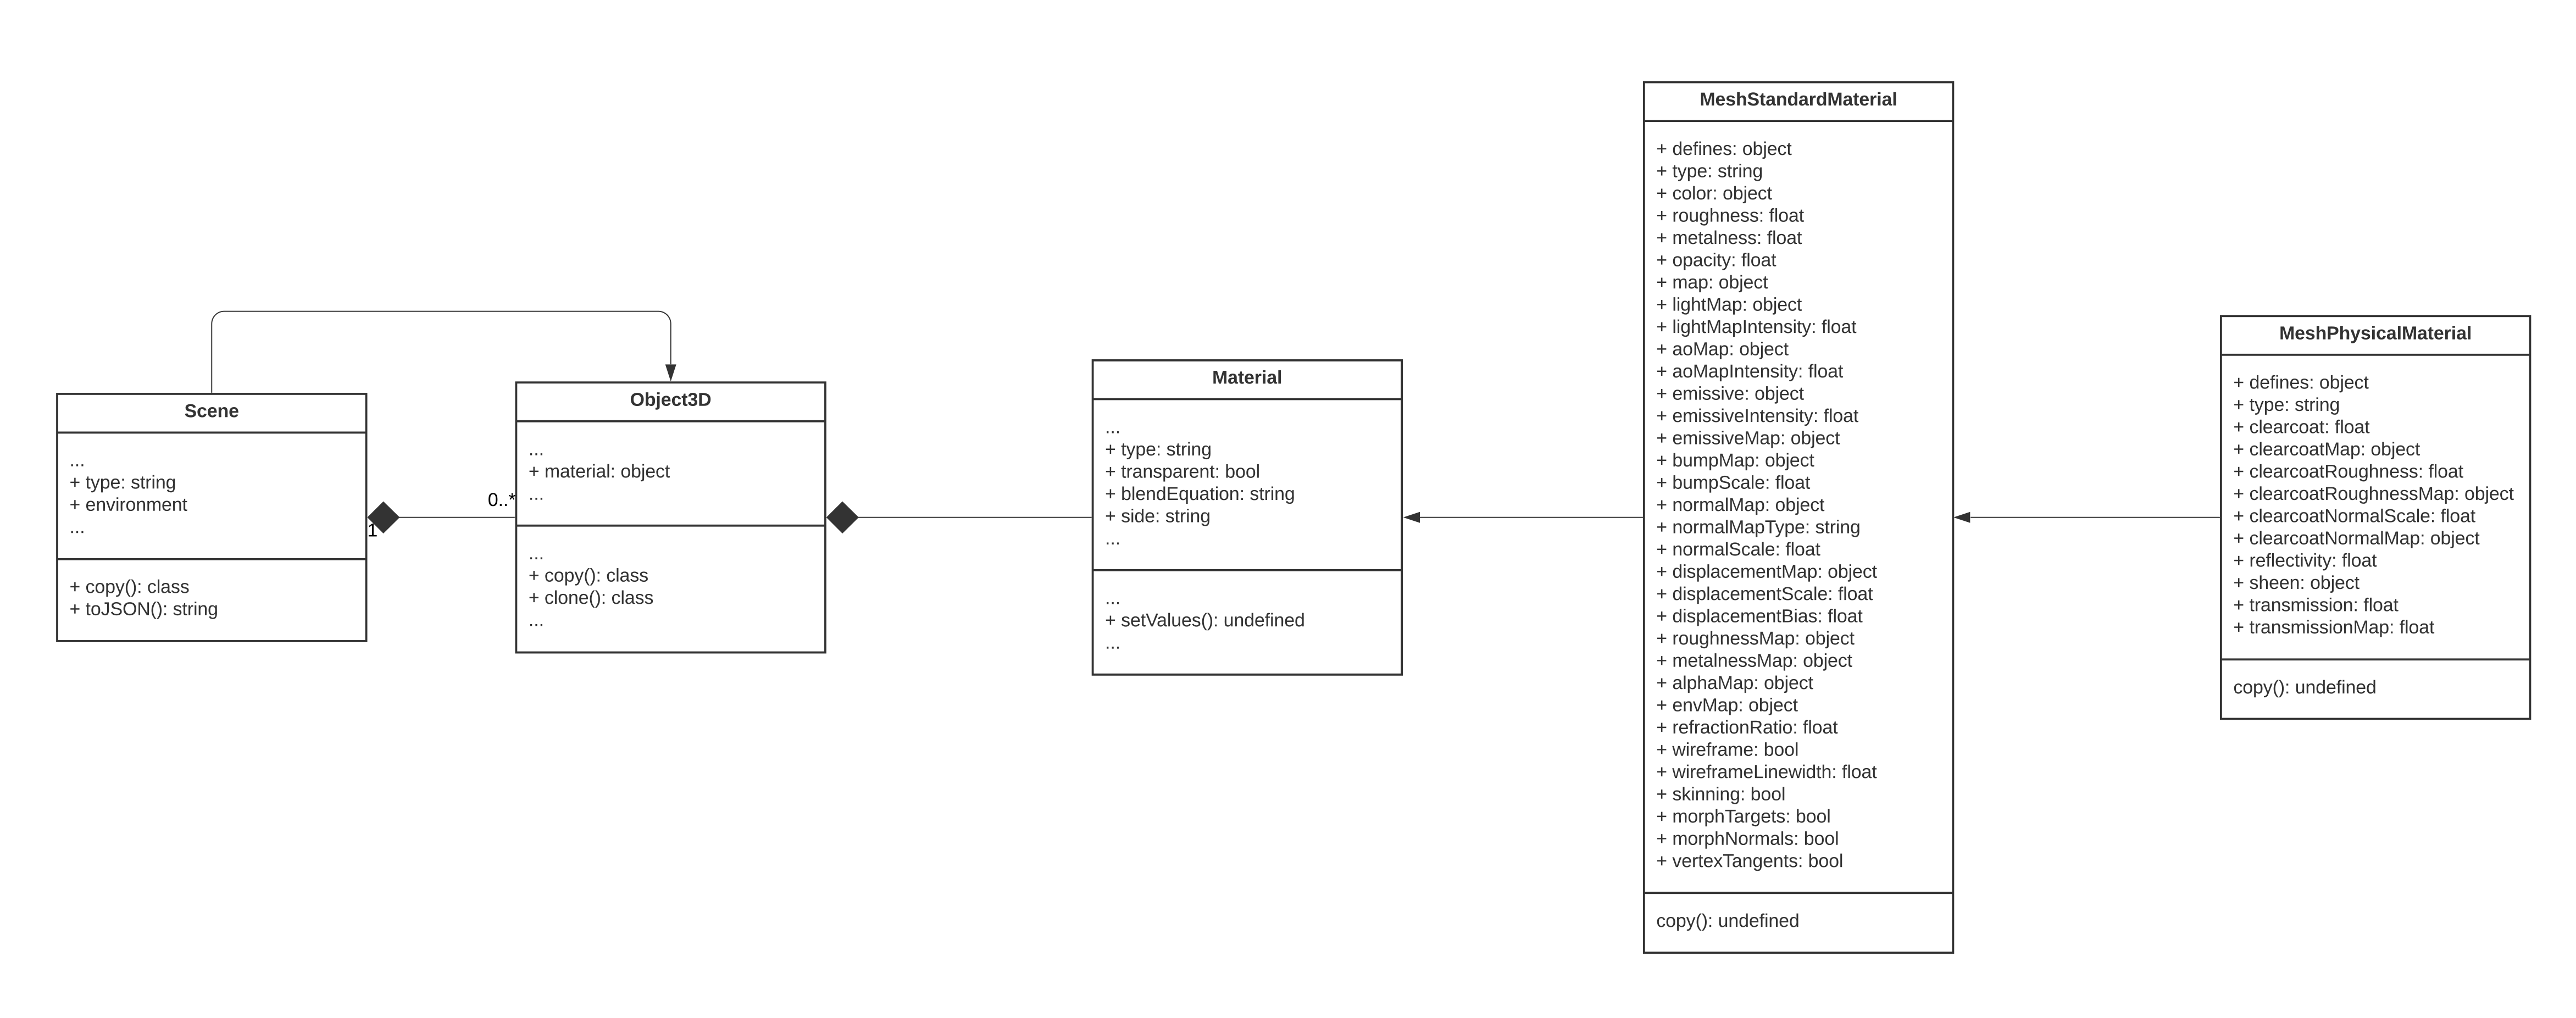
\includegraphics[scale=0.35]{threejs_scenegraph}}
  \caption{Documentaci\'on de los recursos SurfaceMaterial y TextureStack en Swagger.}
  \vspace{0.5cm}
\end{figure}

La clase base de la que heredan es \textit{Material} y almacena informaci\'on com\'un
cualquier tipo de material: opacidad, ecuaci\'on de blending, la cara visible, etc. Adem\'as proporciona un m\'etodo
para configurar los valores de las propiedades del material, as\'i como m\'etodos para la copia, clonado o serializaci\'on
del material.\\

\textit{MeshStandarMaterial} hereda de \textit{Material} y es la implementaci\'on base de un material PBR. Almacena propiedades comunes
como el color el mapa de normales, mapa de desplazamiento, adem\'as de sobreescribir la parametrizaci\'on de shaders y la funci\'on de \textit{copy} de la clase \textit{Material} para copiar correctamente
estas nuevas propiedades.\\

El \textit{MeshPhysicalMaterial} hereda de \textit{MeshStandarMaterial} an\~adiendo el l\'obulo de \textit{clearcoat} y
el BRDF alternativo para el \textit{sheen}, utiliza sus propia parametrizaci\'on de shaders y sobreescribe la funci\'on de copia.\\

Los elementos que se renderizan en la escena, heredan de la clase base \textit{Object3D}, que guarda una referencia o varias
referencias a materiales. El grafo de escena se gestiona desde la clase \textit{Scene}, que hereda de \textit{Object3D} y guarda
informaci\'on sobre el fondo o mapa de entorno, adem\'as de proporcionar sus propios m\'etodos de copia y serializaci\'on
a JSON.

\begin{figure}[H]
  \centering
    \frame{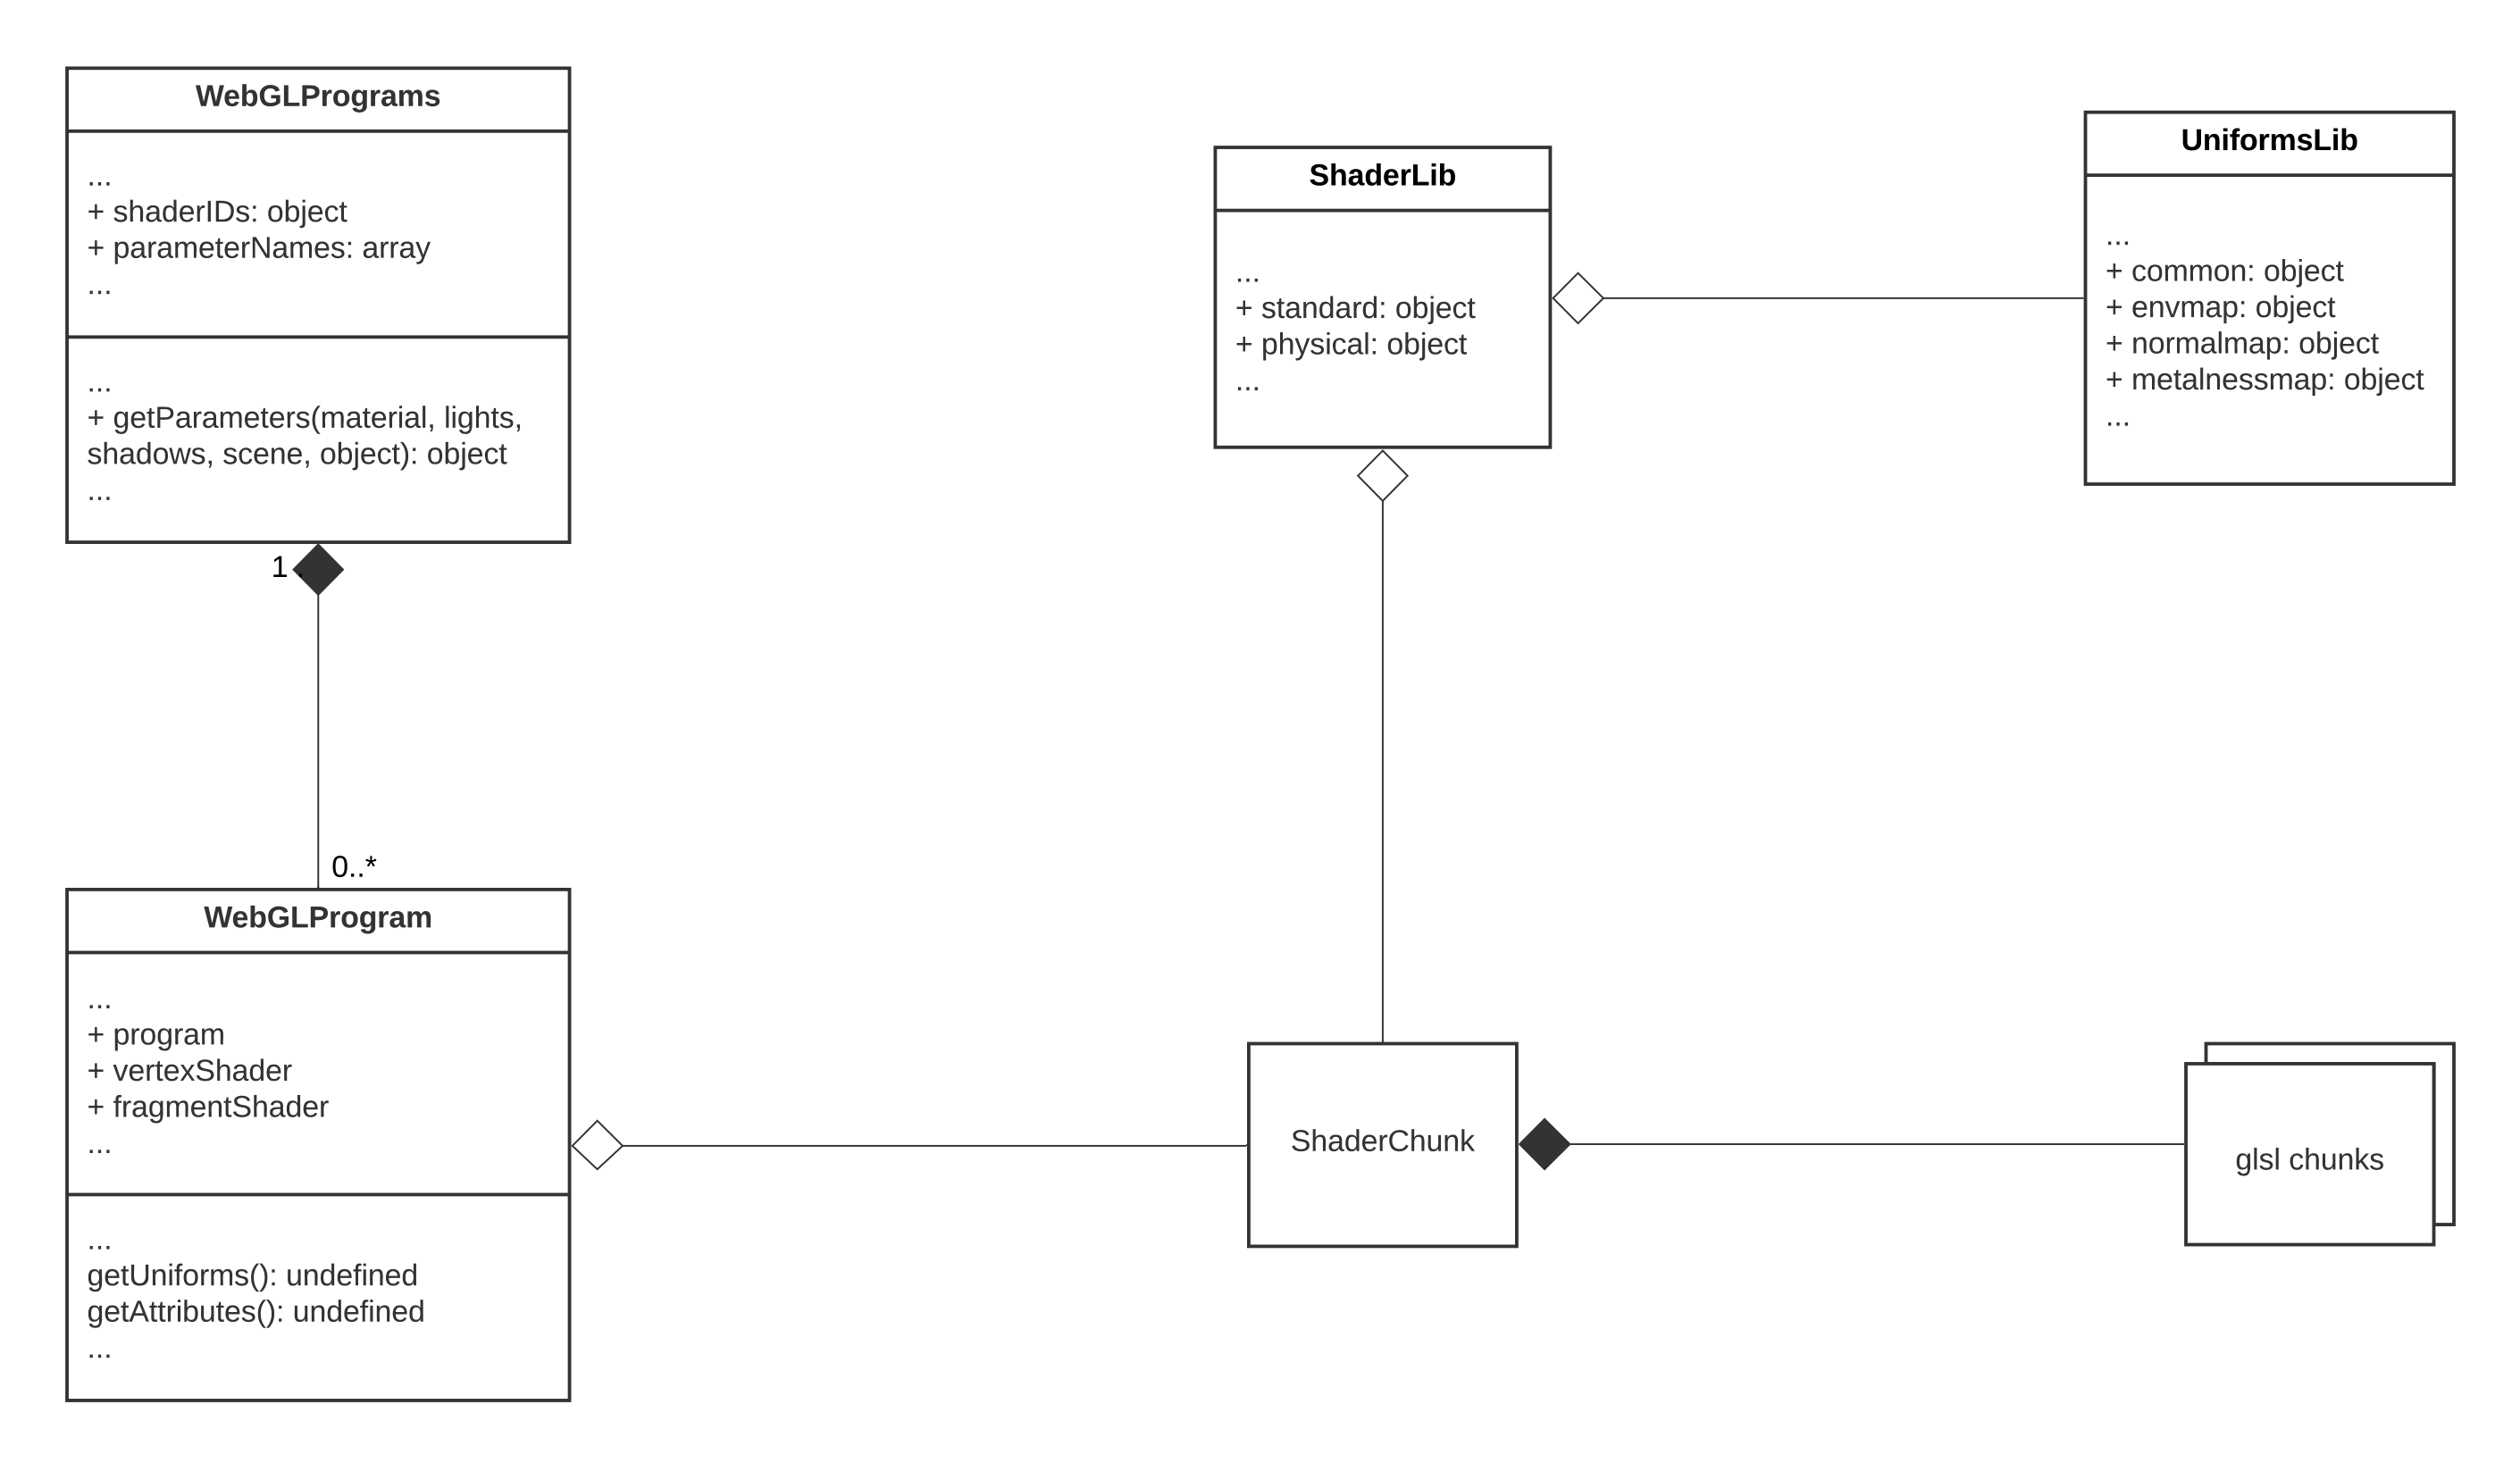
\includegraphics[scale=0.37]{threejs_webglprogram}}
  \caption{Estructuras de datos de ThreeJs que se encargan de la gesti\'on de programas de WebGL}
  \vspace{0.5cm}
\end{figure}

Para generar los \textit{WebGLProgram} del API de WebGL, ThreeJs organiza el c\'odigo GLSL en \textit{chunks}, o trozos de c\'odigo
que se reutilizan y se componen en tiempo de ejecuci\'on para generar el c\'odigo del programa de WebGL.\\

De la misma forma, los \textit{uniforms} que se reutilizan entre programas se organizan en el objeto \textit{UniformsLib}. El objeto ShaderLib almacena
los materiales est\'andar de la librer\'ia, \textit{MeshStandardMaterial}, \textit{MeshPhysicalMaterial}, etc, utilizando los trozos
de c\'odigo GLSL de \textit{ShaderChunk}, los uniforms definidos en \textit{UniformsLib}, adem\'as de los \textit{uniforms} \'unicos
para cada tipo de material.\\

La clase \textit{WebGLProgram} se encarga de juntar los trozos de c\'odigo GLSL y generar la cadena de texto que se utilizar\'a en
el programa WebGL. Las instancias de la clase \textit{WebGLProgram} se cachean en una lista de referencias en \textit{WebGLPrograms}, que proporciona
acceso a la lista, as\'i como funciones para actualizarla u obtener los par\'ametros o los \textit{uniforms} de un programa. \\

Finalmente, la clase \textit{WebGLRenderer} es donde se gestiona la l\'ogica del motor de render y se orquesta la relaci\'on entre todos
estos componentes. \textit{WebGLRenderer} recibe una referencia al grafo de escena, la clase \textit{Scene}, que se encarga de inicializar
y actualizar todos los materiales de la escena, referenciados en la clase base de cualquier elemento que se renderiza en la escena, \textit{Object3D}.
Tiene una referencia a \textit{WebGLMaterials}, que ofrece un m\'etodo para actualizar los \textit{uniforms} de cualquier tipo
de los materiales nativos de ThreeJs.

% Todos los programas GLSL se gestionan desde WebGLPrograms, un closure que contiene un lista de \textit{ids} de los materiales
% nativos de la librer\'ia y otra lista de todos los posibles par\'ametros de \'estos materiales. Cachea los programas utilizados
% en la aplicaci\'on y propociona m\'etodos para obtener los par\'ametros de un material, obtener sus uniforms, cachear un programa,
% obtener un programa o generarlo en caso de que no exista, o borrarlo. WebGLPrograms almacena instancias de la clase WebGLProgram




\subsection{Materiales PBR en ThreeJs}
ThreeJs presenta desde su versi\'on 74 el material \textit{MeshStandardMaterial}, basado en f\'isica y desde la versi\'on
76, el \textit{MeshPhysicalMaterial}, que extiende al anterior a\~nadiendo par\'ametros presentes en el modelo de Disney.
El modelo est\'a basado en el de Disney 2012 \autocite{disney12}, pero con algunas diferencias con intenci\'on de hacerlo m\'as ligero
para la plataforma web. A continuaci\'on se detallan los principales cambios entre los dos modelos:

  \subsubsection{Componente difusa}
  Al contrario que en Disney, el modelo de ThreeJs utiliza directamente el modelo de Lambert, considerando una retrodispersi\'on
  uniformemente distribuida en todas direcciones.\\

  Componente difusa en ThreeJs:

  \begin{equation}
    f_d = \frac{c}{\pi}
  \end{equation}
  \singlespacing

  Componente difusa en Disney 2012:

  \begin{equation}
    f_d = \frac{baseColor}{\pi}
    \left(  1 + (F_{D90} - 1)(1 - cos\theta_{wi})^5  \right)
    \left(  1 + (F_{D90} - 1)(1 - cos\theta_{wo})^5  \right)
  \end{equation}
  \singlespacing


  \subsubsection{Componente especular}
  El BRDF del l\'obulo primario es siempre isotr\'opico, a diferencia del de Disney 2012 \autocite{disney12}, en el que
  el l\'obulo primario puede ser isotr\'opico o anistr\'opico, al contrario que el l\'obulo de \textit{clearcoat},
  que siempre es isotr\'opico. Adem\'as el especular utiliza un BRDF GGX \autocite{ggx}, a diferencia del GTR \autocite{disney12} del modelo de Disney.
  A continuaci\'on el c\'odigo del BRDF especular en ThreeJs:

  \singlespacing
  \begin{lstlisting}[caption=Clase MeshClothMaterial]
vec3 BRDF_Specular_GGX(
  const in IncidentLight incidentLight,
  const in vec3
  viewDir,
  const in vec3 normal,
  const in vec3
  specularColor,
  const in float roughness
) {
  float alpha = pow2( roughness );
  vec3 halfDir = normalize( incidentLight.direction + viewDir );
  float dotNL = saturate( dot( normal, incidentLight.direction ) );
  float dotNV = saturate( dot( normal, viewDir ) );
  float dotNH = saturate( dot( normal, halfDir ) );
  float dotLH = saturate( dot( incidentLight.direction, halfDir ) );
  vec3 F = F_Schlick( specularColor, dotLH );
  float G = G_GGX_SmithCorrelated( alpha, dotNL, dotNV );
  float D = D_GGX( alpha, dotNH );
  return F * ( G * D );
}
  \end{lstlisting}
  \singlespacing

  \subsection*{T\'ermino D}
  Utiliza una aproximaci\'on de la distribuci\'on GGX, frente a la GTR utilizada en el modelo de Disney, por lo que
  presenta una cola m\'as corta.\\

  Funci\'on de distribuci\'on de las normales en ThreeJs:\\

  \begin{equation}
    D_{GGX}(m) = \frac{\alpha^2}{\pi((n\cdotp{m})^2(\alpha^2 - 1 ) + 1)^2}
  \end{equation}
  \singlespacing

  Funci\'on de distribuci\'on de las normales en Disney 2012:\\

  \begin{equation}
    D_{GTR} = \frac
    {c}
    {(\alpha^2 cos^2 \theta_h + sin^2 \theta_h)^2}
  \end{equation}
  \singlespacing

  \begin{lstlisting}[caption=Implementaci\'on en ThreeJs del t\'ermino de geometr\'ia]
float D_GGX( const in float alpha, const in float dotNH ) {

  float a2 = pow2( alpha );
  float denom = pow2( dotNH ) * ( a2 - 1.0 ) + 1.0;

  return RECIPROCAL_PI * a2 / pow2( denom );
}
  \end{lstlisting}
  \singlespacing

  \subsection*{T\'ermino F}
  Igual que en el modelo de Disney 2012, se considera la funci\'on de Fresnel-Schlick lo suficientemente precisa para
  estimar el Fresnel, sin embargo, en \'este caso se utiliza la aproximaci\'on presentada por Epic en el Siggraph de 2013 \autocite{unreal}.\\

  \begin{equation}
    F= F_0 + (1 - F_0)2^{(-5.55473cos\theta_d - 5.55473cos\theta_d)}
  \end{equation}
  \begin{eqfloat}


  \begin{lstlisting}[caption=Implementaci\'on en ThreeJs de la aproximaci\'on a la funci\'on de Fresnel]
vec3 F_Schlick( const in vec3 specularColor, const in float dotLH ) {

  float fresnel = exp2( ( -5.55473 * dotLH - 6.98316 ) * dotLH );

  return ( 1.0 - specularColor ) * fresnel + specularColor;

}
  \end{lstlisting}

  \subsection*{T\'ermino G}
  Para definir las microfacetas en sombra o enmascaradas, ThreeJs utiliza el mismo t\'ermino que Disney 2012, usa
  la formulaci\'on de Smith para separar la funci\'on en dos componentes, luz y vista, utilizando la misma ecuaci\'on
  para las dos.\\

  $$
  V(w_i, w_o) = \frac{0.5}{V_1(w_i) + V_1(w_o)}
  $$
  \singlespacing
  \begin{equation}
    G_1(w_i) = (n \cdot{w_o}) \sqrt{((-n\cdot{w_i}) \alpha^2 + n\cdot{w_i}) n\cdot{w_i} + \alpha^2}
  \end{equation}



\begin{lstlisting}[caption=Clase MeshClothMaterial]
float G_GGX_SmithCorrelated(
  const in float alpha,
  const in float dotNL,
  const in float dotNV
) {

  float a2 = pow2( alpha );

  float gv = dotNL * sqrt( a2 + ( 1.0 - a2 ) * pow2( dotNV ) );
  float gl = dotNV * sqrt( a2 + ( 1.0 - a2 ) * pow2( dotNL ) );

  return 0.5 / max( gv + gl, EPSILON );

}
\end{lstlisting}

  \subsection*{\textit{Clearcoat}}
  El efecto de \textit{clearcoat}, se utiliza para simular efectos de barniz o recubrimientos, y se aplican tanto en Disney
  2012 como un l\'obulo secundario. Mientras que en ThreeJs se utiliza el mismo BRDF con la misma parametrizaci\'on que para
  el l\'obulo primario, en Disney 2012, var\'ia la parametrizaci\'on de los t\'erminos D y G.\\

  $$
  G_{GGX}(v) = \frac
  {2 (n \cdot{v})}
  {(n \cdot{v}) + \sqrt{ \alpha^2 + (1 - \alpha)^2 (n \cdot{v})^2 }}
  $$
  \begin{eqfloat}[!htb]
    \begin{equation}
    \textrm{siendo}\ \alpha=0.25,\;
    G_{GGX}(v) = \frac
    {2 (n \cdot{v})}
    {(n \cdot{v}) + \sqrt{ 0.0625 + 0.5625 (n \cdot{v})^2 }}
    \end{equation}
  \caption{Funci\'on de geometr\'ia para el l\'obulo de \textit{clearcoat} en ThreeJs}
  \end{eqfloat}
  \singlespacing

  \begin{lstlisting}[caption={Implementaci\'on del l\'obulo de \textit{clearcoat} en ThreeJs}]
void RE_Direct_Physical(
  const in IncidentLight directLight,
  const in GeometricContext geometry,
  const in PhysicalMaterial material,
  inout ReflectedLight reflectedLight
) {

  //...
  #ifdef CLEARCOAT

    // ...
    reflectedLight.directSpecular += ccIrradiance * material.clearcoat
      * BRDF_Specular_GGX(
        directLight,
        geometry.viewDir,
        geometry.clearcoatNormal,
        vec3( DEFAULT_SPECULAR_COEFFICIENT ),
        material.clearcoatRoughness
      );

  #else
  // ...

}
  \end{lstlisting}
  
  \subsection*{\textit{Sheen}}
  El par\'ametro de \textit{sheen} ofrece un mayor control sobre la reflectancia especular, permitiendo crear materiales con
  especulares en dos tonos.\\

  ThreeJs utiliza un BRDF diferente cuando el par\'ametro de \textit{sheen}, mientras que en el modelo de Disney el \textit{sheen}
  se modela como otro l\'obulo adicional adem\'as del de \textit{clearcoat}.\\

  $$
  f(\textit{sheen}, \theta_d) =\frac{D_{Charlie}}{4(n\cdot{l} + n\cdot{v} - (n\cdot{l})(n\cdot{v}) )}
  $$
  \begin{eqfloat}[!htb]
    \begin{equation}
      \textrm{siendo}\ D_{Charlie}(\alpha) = \frac
      {(2 + \frac{1}{\alpha})sin(\theta)^\frac{1}{\alpha}}
      {2\pi}
    \end{equation}
  \caption{Modelo de BRDF utilizando \textit{sheen} en ThreeJs}
  \end{eqfloat}
  \singlespacing

  \begin{eqfloat}[!htb]
    \begin{equation}
      f(\textit{sheen}, \theta_d) = \textit{sheen} * ((1 - \textit{sheenTint}) + \textit{sheenTint} * \textit{tint}) * (1 - \cos\theta_d)^5
    \end{equation}
  \caption{L\'obulo adicional de \textit{sheen} en Disney 2012}
  \end{eqfloat}
  \singlespacing

  \begin{lstlisting}[caption={BRDF del modelo de \textit{sheen} de ThreeJs}]
vec3 BRDF_Specular_Sheen(
  const in float roughness,
  const in vec3 L,
  const in GeometricContext geometry,
  vec3 specularColor
) {

  vec3 N = geometry.normal;
  vec3 V = geometry.viewDir;

  vec3 H = normalize( V + L );
  float dotNH = saturate( dot( N, H ) );

  return specularColor * D_Charlie( roughness, dotNH )
    * V_Neubelt( dot(N, V), dot(N, L) );

}
  \end{lstlisting}